\documentclass{extbook}[14pt]
\usepackage{multicol, enumerate, enumitem, hyperref, color, soul, setspace, parskip, fancyhdr, amssymb, amsthm, amsmath, latexsym, units, mathtools}
\everymath{\displaystyle}
\usepackage[headsep=0.5cm,headheight=0cm, left=1 in,right= 1 in,top= 1 in,bottom= 1 in]{geometry}
\usepackage{dashrule}  % Package to use the command below to create lines between items
\newcommand{\litem}[1]{\item #1

\rule{\textwidth}{0.4pt}}
\pagestyle{fancy}
\lhead{}
\chead{Answer Key for Progress Quiz 10 Version A}
\rhead{}
\lfoot{5170-5105}
\cfoot{}
\rfoot{Summer C 2021}
\begin{document}
\textbf{This key should allow you to understand why you choose the option you did (beyond just getting a question right or wrong). \href{https://xronos.clas.ufl.edu/mac1105spring2020/courseDescriptionAndMisc/Exams/LearningFromResults}{More instructions on how to use this key can be found here}.}

\textbf{If you have a suggestion to make the keys better, \href{https://forms.gle/CZkbZmPbC9XALEE88}{please fill out the short survey here}.}

\textit{Note: This key is auto-generated and may contain issues and/or errors. The keys are reviewed after each exam to ensure grading is done accurately. If there are issues (like duplicate options), they are noted in the offline gradebook. The keys are a work-in-progress to give students as many resources to improve as possible.}

\rule{\textwidth}{0.4pt}

\begin{enumerate}\litem{
Which of the following equations \textit{could} be of the graph presented below?

\begin{center}
    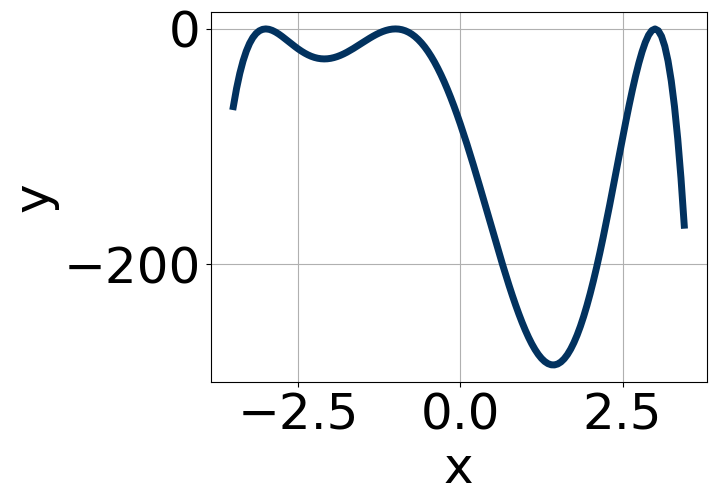
\includegraphics[width=0.5\textwidth]{../Figures/polyGraphToFunctionA.png}
\end{center}


The solution is \( -18(x + 3)^{6} (x + 1)^{4} (x - 3)^{8} \), which is option A.\begin{enumerate}[label=\Alph*.]
\item \( -18(x + 3)^{6} (x + 1)^{4} (x - 3)^{8} \)

* This is the correct option.
\item \( 12(x + 3)^{8} (x + 1)^{4} (x - 3)^{7} \)

The factor $(x - 3)$ should have an even power and the leading coefficient should be the opposite sign.
\item \( -7(x + 3)^{6} (x + 1)^{10} (x - 3)^{7} \)

The factor $(x - 3)$ should have an even power.
\item \( 8(x + 3)^{6} (x + 1)^{6} (x - 3)^{6} \)

This corresponds to the leading coefficient being the opposite value than it should be.
\item \( -12(x + 3)^{10} (x + 1)^{11} (x - 3)^{5} \)

The factors $(x + 1)$ and $(x - 3)$ should both have even powers.
\end{enumerate}

\textbf{General Comment:} General Comments: Draw the x-axis to determine which zeros are touching (and so have even multiplicity) or cross (and have odd multiplicity).
}
\litem{
Describe the end behavior of the polynomial below.
\[ f(x) = -9(x + 8)^{2}(x - 8)^{5}(x - 6)^{2}(x + 6)^{3} \]The solution is the graph below, which is option B.
    \begin{center}
        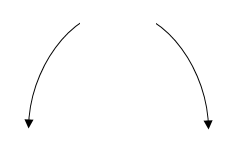
\includegraphics[width=0.3\textwidth]{../Figures/polyEndBehaviorBA.png}
    \end{center}\begin{enumerate}[label=\Alph*.]
\begin{multicols}{2}
\item 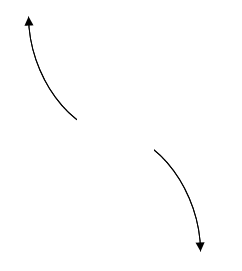
\includegraphics[width = 0.3\textwidth]{../Figures/polyEndBehaviorAA.png}
\item 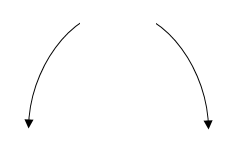
\includegraphics[width = 0.3\textwidth]{../Figures/polyEndBehaviorBA.png}
\item 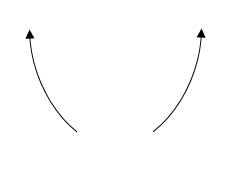
\includegraphics[width = 0.3\textwidth]{../Figures/polyEndBehaviorCA.png}
\item 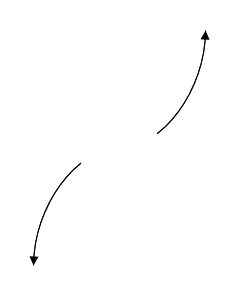
\includegraphics[width = 0.3\textwidth]{../Figures/polyEndBehaviorDA.png}
\end{multicols}\item None of the above.\end{enumerate}
\textbf{General Comment:} Remember that end behavior is determined by the leading coefficient AND whether the \textbf{sum} of the multiplicities is positive or negative.
}
\litem{
Construct the lowest-degree polynomial given the zeros below. Then, choose the intervals that contain the coefficients of the polynomial in the form $x^3+bx^2+cx+d$.
\[ 4 + 3 i \text{ and } 1 \]The solution is \( x^{3} -9 x^{2} +33 x -25 \), which is option C.\begin{enumerate}[label=\Alph*.]
\item \( b \in [1, 2], c \in [-6, -4.35], \text{ and } d \in [3.48, 4.06] \)

$x^{3} + x^{2} -5 x + 4$, which corresponds to multiplying out $(x -4)(x -1)$.
\item \( b \in [1, 2], c \in [-4.24, -2.63], \text{ and } d \in [2.96, 3.37] \)

$x^{3} + x^{2} -4 x + 3$, which corresponds to multiplying out $(x -3)(x -1)$.
\item \( b \in [-17, -7], c \in [31.51, 33.82], \text{ and } d \in [-25.2, -24.86] \)

* $x^{3} -9 x^{2} +33 x -25$, which is the correct option.
\item \( b \in [8, 10], c \in [31.51, 33.82], \text{ and } d \in [24.44, 25.5] \)

$x^{3} +9 x^{2} +33 x + 25$, which corresponds to multiplying out $(x-(4 + 3 i))(x-(4 - 3 i))(x + 1)$.
\item \( \text{None of the above.} \)

This corresponds to making an unanticipated error or not understanding how to use nonreal complex numbers to create the lowest-degree polynomial. If you chose this and are not sure what you did wrong, please contact the coordinator for help.
\end{enumerate}

\textbf{General Comment:} Remember that the conjugate of $a+bi$ is $a-bi$. Since these zeros always come in pairs, we need to multiply out $(x-(4 + 3 i))(x-(4 - 3 i))(x-(1))$.
}
\litem{
Which of the following equations \textit{could} be of the graph presented below?

\begin{center}
    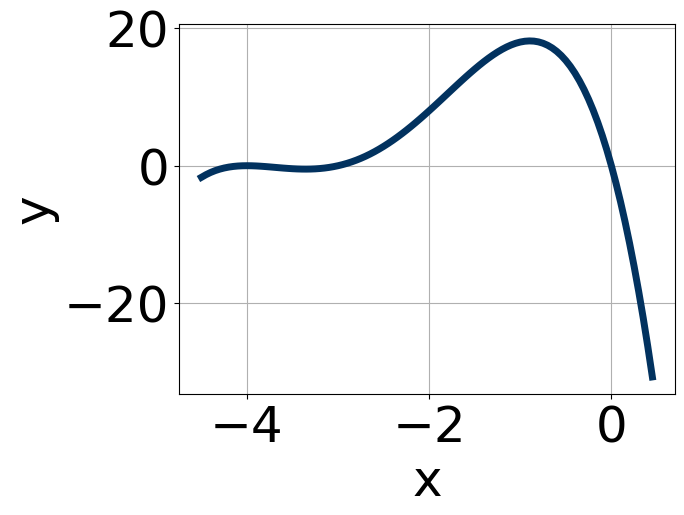
\includegraphics[width=0.5\textwidth]{../Figures/polyGraphToFunctionCopyA.png}
\end{center}


The solution is \( -5x^{5} (x + 4)^{8} (x + 3)^{7} \), which is option A.\begin{enumerate}[label=\Alph*.]
\item \( -5x^{5} (x + 4)^{8} (x + 3)^{7} \)

* This is the correct option.
\item \( -19x^{6} (x + 4)^{6} (x + 3)^{7} \)

The factor $x$ should have an odd power.
\item \( -14x^{10} (x + 4)^{9} (x + 3)^{5} \)

The factor $-4$ should have an even power and the factor $0$ should have an odd power.
\item \( 10x^{11} (x + 4)^{8} (x + 3)^{10} \)

The factor $(x + 3)$ should have an odd power and the leading coefficient should be the opposite sign.
\item \( 19x^{11} (x + 4)^{4} (x + 3)^{7} \)

This corresponds to the leading coefficient being the opposite value than it should be.
\end{enumerate}

\textbf{General Comment:} General Comments: Draw the x-axis to determine which zeros are touching (and so have even multiplicity) or cross (and have odd multiplicity).
}
\litem{
Describe the zero behavior of the zero $x = 8$ of the polynomial below.
\[ f(x) = -9(x - 6)^{9}(x + 6)^{6}(x - 8)^{12}(x + 8)^{9} \]The solution is the graph below, which is option B.
    \begin{center}
        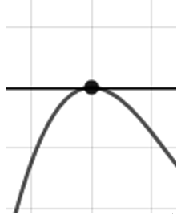
\includegraphics[width=0.3\textwidth]{../Figures/polyZeroBehaviorCopyBA.png}
    \end{center}\begin{enumerate}[label=\Alph*.]
\begin{multicols}{2}
\item 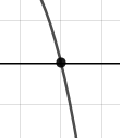
\includegraphics[width = 0.3\textwidth]{../Figures/polyZeroBehaviorCopyAA.png}
\item 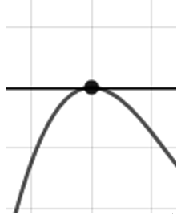
\includegraphics[width = 0.3\textwidth]{../Figures/polyZeroBehaviorCopyBA.png}
\item 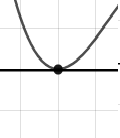
\includegraphics[width = 0.3\textwidth]{../Figures/polyZeroBehaviorCopyCA.png}
\item 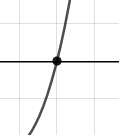
\includegraphics[width = 0.3\textwidth]{../Figures/polyZeroBehaviorCopyDA.png}
\end{multicols}\item None of the above.\end{enumerate}
\textbf{General Comment:} You will need to sketch the entire graph, then zoom in on the zero the question asks about.
}
\litem{
Construct the lowest-degree polynomial given the zeros below. Then, choose the intervals that contain the coefficients of the polynomial in the form $ax^3+bx^2+cx+d$.
\[ \frac{3}{2}, 5, \text{ and } \frac{-4}{3} \]The solution is \( 6x^{3} -31 x^{2} -7 x + 60 \), which is option B.\begin{enumerate}[label=\Alph*.]
\item \( a \in [0, 10], b \in [45, 52], c \in [97, 103], \text{ and } d \in [55, 64] \)

$6x^{3} +47 x^{2} +97 x + 60$, which corresponds to multiplying out $(2x + 3)(x + 5)(3x + 4)$.
\item \( a \in [0, 10], b \in [-34, -27], c \in [-9, -4], \text{ and } d \in [55, 64] \)

* $6x^{3} -31 x^{2} -7 x + 60$, which is the correct option.
\item \( a \in [0, 10], b \in [-34, -27], c \in [-9, -4], \text{ and } d \in [-66, -56] \)

$6x^{3} -31 x^{2} -7 x -60$, which corresponds to multiplying everything correctly except the constant term.
\item \( a \in [0, 10], b \in [26, 37], c \in [-9, -4], \text{ and } d \in [-66, -56] \)

$6x^{3} +31 x^{2} -7 x -60$, which corresponds to multiplying out $(2x + 3)(x + 5)(3x -4)$.
\item \( a \in [0, 10], b \in [-13, -7], c \in [-76, -68], \text{ and } d \in [-66, -56] \)

$6x^{3} -13 x^{2} -73 x -60$, which corresponds to multiplying out $(2x + 3)(x -5)(3x + 4)$.
\end{enumerate}

\textbf{General Comment:} To construct the lowest-degree polynomial, you want to multiply out $(2x -3)(x -5)(3x + 4)$
}
\litem{
Construct the lowest-degree polynomial given the zeros below. Then, choose the intervals that contain the coefficients of the polynomial in the form $x^3+bx^2+cx+d$.
\[ -3 + 2 i \text{ and } 2 \]The solution is \( x^{3} +4 x^{2} +x -26 \), which is option C.\begin{enumerate}[label=\Alph*.]
\item \( b \in [-5.5, -1.2], c \in [-3, 3], \text{ and } d \in [24, 27] \)

$x^{3} -4 x^{2} +x + 26$, which corresponds to multiplying out $(x-(-3 + 2 i))(x-(-3 - 2 i))(x + 2)$.
\item \( b \in [0.7, 1.5], c \in [-6, -3], \text{ and } d \in [0, 9] \)

$x^{3} + x^{2} -4 x + 4$, which corresponds to multiplying out $(x -2)(x -2)$.
\item \( b \in [3.8, 5.3], c \in [-3, 3], \text{ and } d \in [-32, -24] \)

* $x^{3} +4 x^{2} +x -26$, which is the correct option.
\item \( b \in [0.7, 1.5], c \in [-3, 3], \text{ and } d \in [-10, -3] \)

$x^{3} + x^{2} +x -6$, which corresponds to multiplying out $(x + 3)(x -2)$.
\item \( \text{None of the above.} \)

This corresponds to making an unanticipated error or not understanding how to use nonreal complex numbers to create the lowest-degree polynomial. If you chose this and are not sure what you did wrong, please contact the coordinator for help.
\end{enumerate}

\textbf{General Comment:} Remember that the conjugate of $a+bi$ is $a-bi$. Since these zeros always come in pairs, we need to multiply out $(x-(-3 + 2 i))(x-(-3 - 2 i))(x-(2))$.
}
\litem{
Construct the lowest-degree polynomial given the zeros below. Then, choose the intervals that contain the coefficients of the polynomial in the form $ax^3+bx^2+cx+d$.
\[ \frac{-3}{5}, \frac{-7}{2}, \text{ and } \frac{-3}{2} \]The solution is \( 20x^{3} +112 x^{2} +165 x + 63 \), which is option C.\begin{enumerate}[label=\Alph*.]
\item \( a \in [15, 23], b \in [110, 119], c \in [165, 169], \text{ and } d \in [-64, -58] \)

$20x^{3} +112 x^{2} +165 x -63$, which corresponds to multiplying everything correctly except the constant term.
\item \( a \in [15, 23], b \in [-117, -109], c \in [165, 169], \text{ and } d \in [-64, -58] \)

$20x^{3} -112 x^{2} +165 x -63$, which corresponds to multiplying out $(5x -3)(2x -7)(2x -3)$.
\item \( a \in [15, 23], b \in [110, 119], c \in [165, 169], \text{ and } d \in [54, 68] \)

* $20x^{3} +112 x^{2} +165 x + 63$, which is the correct option.
\item \( a \in [15, 23], b \in [-53, -49], c \in [-85, -80], \text{ and } d \in [54, 68] \)

$20x^{3} -52 x^{2} -81 x + 63$, which corresponds to multiplying out $(5x -3)(2x -7)(2x + 3)$.
\item \( a \in [15, 23], b \in [88, 93], c \in [36, 51], \text{ and } d \in [-64, -58] \)

$20x^{3} +88 x^{2} +45 x -63$, which corresponds to multiplying out $(5x -3)(2x + 7)(2x + 3)$.
\end{enumerate}

\textbf{General Comment:} To construct the lowest-degree polynomial, you want to multiply out $(5x + 3)(2x + 7)(2x + 3)$
}
\litem{
Describe the zero behavior of the zero $x = 7$ of the polynomial below.
\[ f(x) = 2(x + 7)^{7}(x - 7)^{10}(x - 3)^{4}(x + 3)^{8} \]The solution is the graph below, which is option C.
    \begin{center}
        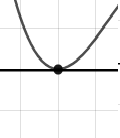
\includegraphics[width=0.3\textwidth]{../Figures/polyZeroBehaviorCA.png}
    \end{center}\begin{enumerate}[label=\Alph*.]
\begin{multicols}{2}
\item 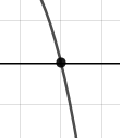
\includegraphics[width = 0.3\textwidth]{../Figures/polyZeroBehaviorAA.png}
\item 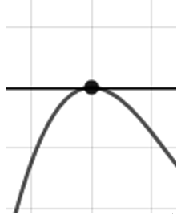
\includegraphics[width = 0.3\textwidth]{../Figures/polyZeroBehaviorBA.png}
\item 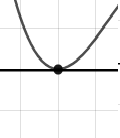
\includegraphics[width = 0.3\textwidth]{../Figures/polyZeroBehaviorCA.png}
\item 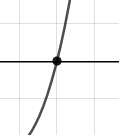
\includegraphics[width = 0.3\textwidth]{../Figures/polyZeroBehaviorDA.png}
\end{multicols}\item None of the above.\end{enumerate}
\textbf{General Comment:} You will need to sketch the entire graph, then zoom in on the zero the question asks about.
}
\litem{
Describe the end behavior of the polynomial below.
\[ f(x) = -3(x + 4)^{3}(x - 4)^{6}(x - 5)^{5}(x + 5)^{7} \]The solution is the graph below, which is option A.
    \begin{center}
        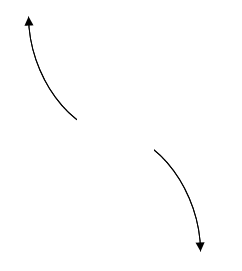
\includegraphics[width=0.3\textwidth]{../Figures/polyEndBehaviorCopyAA.png}
    \end{center}\begin{enumerate}[label=\Alph*.]
\begin{multicols}{2}
\item 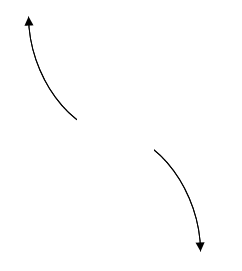
\includegraphics[width = 0.3\textwidth]{../Figures/polyEndBehaviorCopyAA.png}
\item 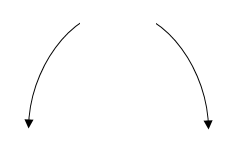
\includegraphics[width = 0.3\textwidth]{../Figures/polyEndBehaviorCopyBA.png}
\item 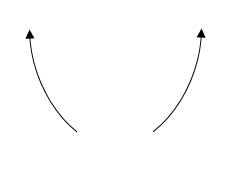
\includegraphics[width = 0.3\textwidth]{../Figures/polyEndBehaviorCopyCA.png}
\item 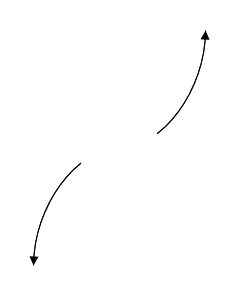
\includegraphics[width = 0.3\textwidth]{../Figures/polyEndBehaviorCopyDA.png}
\end{multicols}\item None of the above.\end{enumerate}
\textbf{General Comment:} Remember that end behavior is determined by the leading coefficient AND whether the \textbf{sum} of the multiplicities is positive or negative.
}
\end{enumerate}

\end{document}